\chapter{Phân tích trừ dần}

\index{phân tích trừ dần}

Độ phức tạp thời gian của một thuật toán
thường dễ dàng phân tích
chỉ bằng cách kiểm tra cấu trúc
của thuật toán:
thuật toán chứa những vòng lặp nào
và các vòng lặp được thực hiện bao nhiêu lần.
Tuy nhiên, đôi khi một phân tích trực tiếp
không mang lại bức tranh chân thực về hiệu quả của thuật toán.

\key{Phân tích trừ dần} (Amortized analysis) có thể được sử dụng để phân tích
các thuật toán chứa các thao tác mà
độ phức tạp thời gian của chúng thay đổi.
Ý tưởng là ước tính tổng thời gian được sử dụng cho
tất cả các thao tác như vậy trong suốt
quá trình thực thi của thuật toán, thay vì tập trung
vào các thao tác riêng lẻ.

\section{Phương pháp hai con trỏ}

\index{phương pháp hai con trỏ}

Trong \key{phương pháp hai con trỏ} (two pointers method),
hai con trỏ được sử dụng để
lặp qua các giá trị của mảng.
Cả hai con trỏ chỉ có thể di chuyển theo một hướng,
điều này đảm bảo rằng thuật toán hoạt động hiệu quả.
Tiếp theo chúng ta sẽ thảo luận về hai bài toán có thể được giải quyết
bằng phương pháp hai con trỏ.

\subsubsection{Tổng của mảng con}

Ví dụ đầu tiên,
hãy xem xét một bài toán mà chúng ta
được cho một mảng gồm $n$ số nguyên dương
và một tổng mục tiêu $x$,
và chúng ta muốn tìm một mảng con có tổng là $x$
hoặc báo cáo rằng không có mảng con nào như vậy.

Ví dụ, mảng
\begin{center}
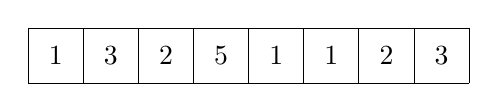
\begin{tikzpicture}[scale=0.7]
\draw (0,0) grid (8,1);

\node at (0.5,0.5) {$1$};
\node at (1.5,0.5) {$3$};
\node at (2.5,0.5) {$2$};
\node at (3.5,0.5) {$5$};
\node at (4.5,0.5) {$1$};
\node at (5.5,0.5) {$1$};
\node at (6.5,0.5) {$2$};
\node at (7.5,0.5) {$3$};
\end{tikzpicture}
\end{center}
chứa một mảng con có tổng là 8:
\begin{center}
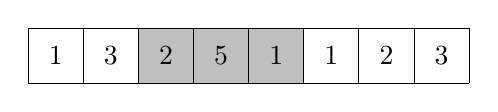
\begin{tikzpicture}[scale=0.7]
\fill[color=lightgray] (2,0) rectangle (5,1);
\draw (0,0) grid (8,1);

\node at (0.5,0.5) {$1$};
\node at (1.5,0.5) {$3$};
\node at (2.5,0.5) {$2$};
\node at (3.5,0.5) {$5$};
\node at (4.5,0.5) {$1$};
\node at (5.5,0.5) {$1$};
\node at (6.5,0.5) {$2$};
\node at (7.5,0.5) {$3$};
\end{tikzpicture}
\end{center}

Bài toán này có thể được giải quyết trong
thời gian $O(n)$ bằng cách sử dụng phương pháp hai con trỏ.
Ý tưởng là duy trì các con trỏ trỏ đến
giá trị đầu tiên và cuối cùng của một mảng con.
Ở mỗi lượt, con trỏ trái di chuyển một bước
sang phải, và con trỏ phải di chuyển sang phải
miễn là tổng của mảng con kết quả không vượt quá $x$.
Nếu tổng trở thành chính xác là $x$,
một giải pháp đã được tìm thấy.

Ví dụ, hãy xem xét mảng sau
và tổng mục tiêu $x=8$:
\begin{center}
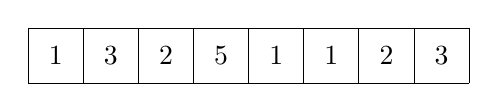
\begin{tikzpicture}[scale=0.7]
\draw (0,0) grid (8,1);

\node at (0.5,0.5) {$1$};
\node at (1.5,0.5) {$3$};
\node at (2.5,0.5) {$2$};
\node at (3.5,0.5) {$5$};
\node at (4.5,0.5) {$1$};
\node at (5.5,0.5) {$1$};
\node at (6.5,0.5) {$2$};
\node at (7.5,0.5) {$3$};
\end{tikzpicture}
\end{center}

Mảng con ban đầu chứa các giá trị
1, 3 và 2 có tổng là 6:

\begin{center}
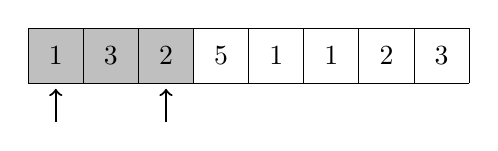
\begin{tikzpicture}[scale=0.7]
\fill[color=lightgray] (0,0) rectangle (3,1);
\draw (0,0) grid (8,1);

\node at (0.5,0.5) {$1$};
\node at (1.5,0.5) {$3$};
\node at (2.5,0.5) {$2$};
\node at (3.5,0.5) {$5$};
\node at (4.5,0.5) {$1$};
\node at (5.5,0.5) {$1$};
\node at (6.5,0.5) {$2$};
\node at (7.5,0.5) {$3$};

\draw[thick,->] (0.5,-0.7) -- (0.5,-0.1);
\draw[thick,->] (2.5,-0.7) -- (2.5,-0.1);
\end{tikzpicture}
\end{center}

Sau đó, con trỏ trái di chuyển một bước sang phải.
Con trỏ phải không di chuyển, bởi vì nếu không
tổng của mảng con sẽ vượt quá $x$.

\begin{center}
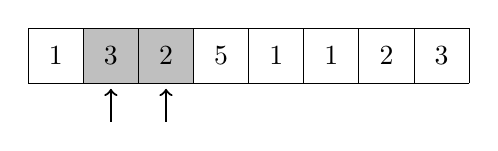
\begin{tikzpicture}[scale=0.7]
\fill[color=lightgray] (1,0) rectangle (3,1);
\draw (0,0) grid (8,1);

\node at (0.5,0.5) {$1$};
\node at (1.5,0.5) {$3$};
\node at (2.5,0.5) {$2$};
\node at (3.5,0.5) {$5$};
\node at (4.5,0.5) {$1$};
\node at (5.5,0.5) {$1$};
\node at (6.5,0.5) {$2$};
\node at (7.5,0.5) {$3$};

\draw[thick,->] (1.5,-0.7) -- (1.5,-0.1);
\draw[thick,->] (2.5,-0.7) -- (2.5,-0.1);
\end{tikzpicture}
\end{center}

Một lần nữa, con trỏ trái di chuyển một bước sang phải,
và lần này con trỏ phải di chuyển ba
bước sang phải.
Tổng của mảng con là $2+5+1=8$, vì vậy một mảng con
có tổng là $x$ đã được tìm thấy.

\begin{center}
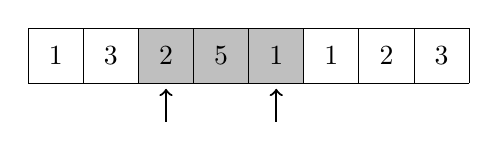
\begin{tikzpicture}[scale=0.7]
\fill[color=lightgray] (2,0) rectangle (5,1);
\draw (0,0) grid (8,1);

\node at (0.5,0.5) {$1$};
\node at (1.5,0.5) {$3$};
\node at (2.5,0.5) {$2$};
\node at (3.5,0.5) {$5$};
\node at (4.5,0.5) {$1$};
\node at (5.5,0.5) {$1$};
\node at (6.5,0.5) {$2$};
\node at (7.5,0.5) {$3$};

\draw[thick,->] (2.5,-0.7) -- (2.5,-0.1);
\draw[thick,->] (4.5,-0.7) -- (4.5,-0.1);
\end{tikzpicture}
\end{center}

Thời gian chạy của thuật toán phụ thuộc vào
số bước mà con trỏ phải di chuyển.
Mặc dù không có giới hạn trên hữu ích nào về số bước mà
con trỏ có thể di chuyển trong một lượt \emph{đơn lẻ},
chúng ta biết rằng con trỏ di chuyển \emph{tổng cộng}
$O(n)$ bước trong suốt thuật toán,
bởi vì nó chỉ di chuyển sang phải.

Vì cả con trỏ trái và phải
đều di chuyển $O(n)$ bước trong suốt thuật toán,
thuật toán hoạt động trong thời gian $O(n)$.

\subsubsection{Bài toán 2SUM}

\index{Bài toán 2SUM}

Một bài toán khác có thể được giải quyết bằng
phương pháp hai con trỏ là bài toán sau,
còn được biết đến với tên gọi \key{bài toán 2SUM}:
cho một mảng gồm $n$ số và
một tổng mục tiêu $x$, hãy tìm
hai giá trị trong mảng sao cho tổng của chúng là $x$,
hoặc báo cáo rằng không tồn tại các giá trị như vậy.

Để giải quyết bài toán, trước tiên chúng ta
sắp xếp các giá trị trong mảng theo thứ tự tăng dần.
Sau đó, chúng ta lặp qua mảng bằng
hai con trỏ.
Con trỏ trái bắt đầu tại giá trị đầu tiên
và di chuyển một bước sang phải ở mỗi lượt.
Con trỏ phải bắt đầu tại giá trị cuối cùng
và luôn di chuyển sang trái cho đến khi tổng của
giá trị ở con trỏ trái và phải không vượt quá $x$.
Nếu tổng chính xác là $x$,
một giải pháp đã được tìm thấy.

Ví dụ, hãy xem xét mảng sau
và tổng mục tiêu $x=12$:
\begin{center}
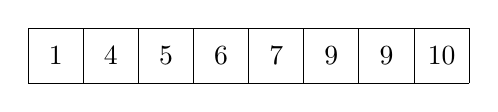
\begin{tikzpicture}[scale=0.7]
\draw (0,0) grid (8,1);

\node at (0.5,0.5) {$1$};
\node at (1.5,0.5) {$4$};
\node at (2.5,0.5) {$5$};
\node at (3.5,0.5) {$6$};
\node at (4.5,0.5) {$7$};
\node at (5.5,0.5) {$9$};
\node at (6.5,0.5) {$9$};
\node at (7.5,0.5) {$10$};
\end{tikzpicture}
\end{center}

Vị trí ban đầu của các con trỏ
như sau.
Tổng của các giá trị là $1+10=11$
nhỏ hơn $x$.

\begin{center}
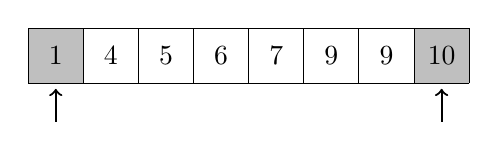
\begin{tikzpicture}[scale=0.7]
\fill[color=lightgray] (0,0) rectangle (1,1);
\fill[color=lightgray] (7,0) rectangle (8,1);
\draw (0,0) grid (8,1);

\node at (0.5,0.5) {$1$};
\node at (1.5,0.5) {$4$};
\node at (2.5,0.5) {$5$};
\node at (3.5,0.5) {$6$};
\node at (4.5,0.5) {$7$};
\node at (5.5,0.5) {$9$};
\node at (6.5,0.5) {$9$};
\node at (7.5,0.5) {$10$};

\draw[thick,->] (0.5,-0.7) -- (0.5,-0.1);
\draw[thick,->] (7.5,-0.7) -- (7.5,-0.1);
\end{tikzpicture}
\end{center}

Sau đó con trỏ trái di chuyển một bước sang phải.
Con trỏ phải di chuyển ba bước sang trái,
và tổng trở thành $4+7=11$.

\begin{center}
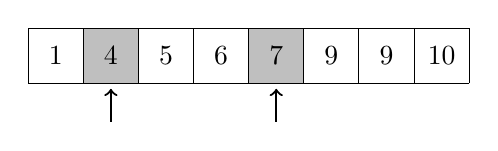
\begin{tikzpicture}[scale=0.7]
\fill[color=lightgray] (1,0) rectangle (2,1);
\fill[color=lightgray] (4,0) rectangle (5,1);
\draw (0,0) grid (8,1);

\node at (0.5,0.5) {$1$};
\node at (1.5,0.5) {$4$};
\node at (2.5,0.5) {$5$};
\node at (3.5,0.5) {$6$};
\node at (4.5,0.5) {$7$};
\node at (5.5,0.5) {$9$};
\node at (6.5,0.5) {$9$};
\node at (7.5,0.5) {$10$};

\draw[thick,->] (1.5,-0.7) -- (1.5,-0.1);
\draw[thick,->] (4.5,-0.7) -- (4.5,-0.1);
\end{tikzpicture}
\end{center}

Sau đó, con trỏ trái lại di chuyển một bước sang phải.
Con trỏ phải không di chuyển, và một giải pháp
$5+7=12$ đã được tìm thấy.

\begin{center}
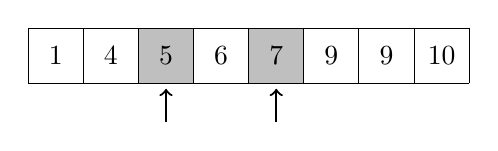
\begin{tikzpicture}[scale=0.7]
\fill[color=lightgray] (2,0) rectangle (3,1);
\fill[color=lightgray] (4,0) rectangle (5,1);
\draw (0,0) grid (8,1);

\node at (0.5,0.5) {$1$};
\node at (1.5,0.5) {$4$};
\node at (2.5,0.5) {$5$};
\node at (3.5,0.5) {$6$};
\node at (4.5,0.5) {$7$};
\node at (5.5,0.5) {$9$};
\node at (6.5,0.5) {$9$};
\node at (7.5,0.5) {$10$};

\draw[thick,->] (2.5,-0.7) -- (2.5,-0.1);
\draw[thick,->] (4.5,-0.7) -- (4.5,-0.1);
\end{tikzpicture}
\end{center}

Thời gian chạy của thuật toán là
$O(n \log n)$, bởi vì nó trước tiên sắp xếp
mảng trong thời gian $O(n \log n)$,
và sau đó cả hai con trỏ di chuyển $O(n)$ bước.

Lưu ý rằng có thể giải quyết bài toán
theo một cách khác trong thời gian $O(n \log n)$ bằng cách sử dụng tìm kiếm nhị phân.
Trong giải pháp như vậy, chúng ta lặp qua mảng
và với mỗi giá trị của mảng, chúng ta cố gắng tìm một
giá trị khác tạo ra tổng $x$.
Điều này có thể được thực hiện bằng cách thực hiện $n$ lần tìm kiếm nhị phân,
mỗi lần mất thời gian $O(\log n)$.

\index{Bài toán 3SUM}
Một bài toán khó hơn là
\key{bài toán 3SUM} yêu cầu tìm
\emph{ba} giá trị trong mảng
có tổng là $x$.
Sử dụng ý tưởng của thuật toán trên,
bài toán này có thể được giải quyết trong thời gian $O(n^2)$\footnote{Trong một thời gian dài,
người ta cho rằng việc giải quyết
bài toán 3SUM hiệu quả hơn $O(n^2)$
là không thể.
Tuy nhiên, vào năm 2014, hóa ra \cite{gro14}
điều này không đúng.}.
Bạn có thấy cách làm không?

\section{Phần tử nhỏ hơn gần nhất}

\index{phần tử nhỏ hơn gần nhất}

Phân tích trừ dần thường được sử dụng để
ước tính số lượng các thao tác
được thực hiện trên một cấu trúc dữ liệu.
Các thao tác có thể được phân bổ không đồng đều sao cho
hầu hết các thao tác xảy ra trong một
giai đoạn nhất định của thuật toán, nhưng tổng
số lượng các thao tác bị giới hạn.

Ví dụ, hãy xem xét bài toán
tìm cho mỗi phần tử của mảng
\key{phần tử nhỏ hơn gần nhất}, tức là,
phần tử nhỏ hơn đầu tiên đứng trước phần tử đó
trong mảng.
Có thể không tồn tại phần tử nào như vậy,
trong trường hợp đó thuật toán nên báo cáo điều này.
Tiếp theo chúng ta sẽ xem làm thế nào bài toán có thể được
giải quyết một cách hiệu quả bằng cách sử dụng cấu trúc ngăn xếp.

Chúng ta duyệt qua mảng từ trái sang phải
và duy trì một ngăn xếp các phần tử của mảng.
Tại mỗi vị trí trong mảng, chúng ta loại bỏ các phần tử khỏi ngăn xếp
cho đến khi phần tử trên đỉnh nhỏ hơn
phần tử hiện tại, hoặc ngăn xếp trống.
Sau đó, chúng ta báo cáo rằng phần tử trên đỉnh là
phần tử nhỏ hơn gần nhất của phần tử hiện tại,
hoặc nếu ngăn xếp trống, không có phần tử nào như vậy.
Cuối cùng, chúng ta thêm phần tử hiện tại vào ngăn xếp.

Ví dụ, hãy xem xét mảng sau:
\begin{center}
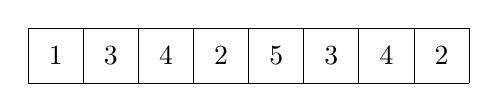
\begin{tikzpicture}[scale=0.7]
\draw (0,0) grid (8,1);

\node at (0.5,0.5) {$1$};
\node at (1.5,0.5) {$3$};
\node at (2.5,0.5) {$4$};
\node at (3.5,0.5) {$2$};
\node at (4.5,0.5) {$5$};
\node at (5.5,0.5) {$3$};
\node at (6.5,0.5) {$4$};
\node at (7.5,0.5) {$2$};
\end{tikzpicture}
\end{center}

Đầu tiên, các phần tử 1, 3 và 4 được thêm vào ngăn xếp,
bởi vì mỗi phần tử lớn hơn phần tử trước đó.
Do đó, phần tử nhỏ hơn gần nhất của 4 là 3,
và phần tử nhỏ hơn gần nhất của 3 là 1.
\begin{center}
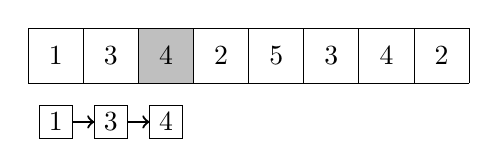
\begin{tikzpicture}[scale=0.7]
\fill[color=lightgray] (2,0) rectangle (3,1);
\draw (0,0) grid (8,1);

\node at (0.5,0.5) {$1$};
\node at (1.5,0.5) {$3$};
\node at (2.5,0.5) {$4$};
\node at (3.5,0.5) {$2$};
\node at (4.5,0.5) {$5$};
\node at (5.5,0.5) {$3$};
\node at (6.5,0.5) {$4$};
\node at (7.5,0.5) {$2$};

\draw (0.2,0.2-1.2) rectangle (0.8,0.8-1.2);
\draw (1.2,0.2-1.2) rectangle (1.8,0.8-1.2);
\draw (2.2,0.2-1.2) rectangle (2.8,0.8-1.2);

\node at (0.5,0.5-1.2) {$1$};
\node at (1.5,0.5-1.2) {$3$};
\node at (2.5,0.5-1.2) {$4$};

\draw[->,thick] (0.8,0.5-1.2) -- (1.2,0.5-1.2);
\draw[->,thick] (1.8,0.5-1.2) -- (2.2,0.5-1.2);
\end{tikzpicture}
\end{center}

Phần tử tiếp theo 2 nhỏ hơn hai phần tử
trên đỉnh trong ngăn xếp.
Do đó, các phần tử 3 và 4 được loại bỏ khỏi ngăn xếp,
và sau đó phần tử 2 được thêm vào ngăn xếp.
Phần tử nhỏ hơn gần nhất của nó là 1:
\begin{center}
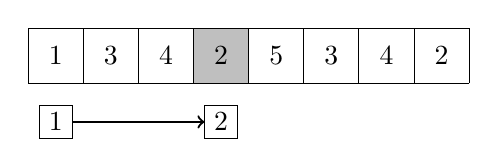
\begin{tikzpicture}[scale=0.7]
\fill[color=lightgray] (3,0) rectangle (4,1);
\draw (0,0) grid (8,1);

\node at (0.5,0.5) {$1$};
\node at (1.5,0.5) {$3$};
\node at (2.5,0.5) {$4$};
\node at (3.5,0.5) {$2$};
\node at (4.5,0.5) {$5$};
\node at (5.5,0.5) {$3$};
\node at (6.5,0.5) {$4$};
\node at (7.5,0.5) {$2$};

\draw (0.2,0.2-1.2) rectangle (0.8,0.8-1.2);
\draw (3.2,0.2-1.2) rectangle (3.8,0.8-1.2);

\node at (0.5,0.5-1.2) {$1$};
\node at (3.5,0.5-1.2) {$2$};

\draw[->,thick] (0.8,0.5-1.2) -- (3.2,0.5-1.2);
\end{tikzpicture}
\end{center}

Sau đó, phần tử 5 lớn hơn phần tử 2,
vì vậy nó sẽ được thêm vào ngăn xếp, và
phần tử nhỏ hơn gần nhất của nó là 2:
\begin{center}
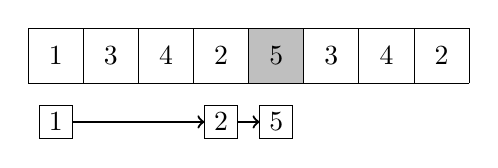
\begin{tikzpicture}[scale=0.7]
\fill[color=lightgray] (4,0) rectangle (5,1);
\draw (0,0) grid (8,1);

\node at (0.5,0.5) {$1$};
\node at (1.5,0.5) {$3$};
\node at (2.5,0.5) {$4$};
\node at (3.5,0.5) {$2$};
\node at (4.5,0.5) {$5$};
\node at (5.5,0.5) {$3$};
\node at (6.5,0.5) {$4$};
\node at (7.5,0.5) {$2$};

\draw (0.2,0.2-1.2) rectangle (0.8,0.8-1.2);
\draw (3.2,0.2-1.2) rectangle (3.8,0.8-1.2);
\draw (4.2,0.2-1.2) rectangle (4.8,0.8-1.2);

\node at (0.5,0.5-1.2) {$1$};
\node at (3.5,0.5-1.2) {$2$};
\node at (4.5,0.5-1.2) {$5$};

\draw[->,thick] (0.8,0.5-1.2) -- (3.2,0.5-1.2);
\draw[->,thick] (3.8,0.5-1.2) -- (4.2,0.5-1.2);
\end{tikzpicture}
\end{center}

Sau đó, phần tử 5 được loại bỏ khỏi ngăn xếp
và các phần tử 3 và 4 được thêm vào ngăn xếp:
\begin{center}
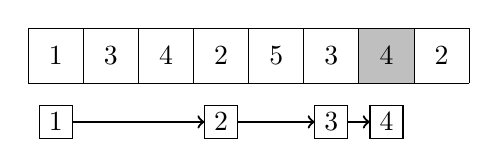
\begin{tikzpicture}[scale=0.7]
\fill[color=lightgray] (6,0) rectangle (7,1);
\draw (0,0) grid (8,1);

\node at (0.5,0.5) {$1$};
\node at (1.5,0.5) {$3$};
\node at (2.5,0.5) {$4$};
\node at (3.5,0.5) {$2$};
\node at (4.5,0.5) {$5$};
\node at (5.5,0.5) {$3$};
\node at (6.5,0.5) {$4$};
\node at (7.5,0.5) {$2$};

\draw (0.2,0.2-1.2) rectangle (0.8,0.8-1.2);
\draw (3.2,0.2-1.2) rectangle (3.8,0.8-1.2);
\draw (5.2,0.2-1.2) rectangle (5.8,0.8-1.2);
\draw (6.2,0.2-1.2) rectangle (6.8,0.8-1.2);

\node at (0.5,0.5-1.2) {$1$};
\node at (3.5,0.5-1.2) {$2$};
\node at (5.5,0.5-1.2) {$3$};
\node at (6.5,0.5-1.2) {$4$};

\draw[->,thick] (0.8,0.5-1.2) -- (3.2,0.5-1.2);
\draw[->,thick] (3.8,0.5-1.2) -- (5.2,0.5-1.2);
\draw[->,thick] (5.8,0.5-1.2) -- (6.2,0.5-1.2);
\end{tikzpicture}
\end{center}

Cuối cùng, tất cả các phần tử ngoại trừ 1 được loại bỏ
khỏi ngăn xếp và phần tử cuối cùng 2
được thêm vào ngăn xếp:

\begin{center}
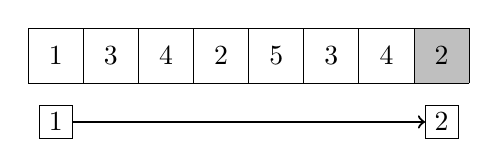
\begin{tikzpicture}[scale=0.7]
\fill[color=lightgray] (7,0) rectangle (8,1);
\draw (0,0) grid (8,1);

\node at (0.5,0.5) {$1$};
\node at (1.5,0.5) {$3$};
\node at (2.5,0.5) {$4$};
\node at (3.5,0.5) {$2$};
\node at (4.5,0.5) {$5$};
\node at (5.5,0.5) {$3$};
\node at (6.5,0.5) {$4$};
\node at (7.5,0.5) {$2$};

\draw (0.2,0.2-1.2) rectangle (0.8,0.8-1.2);
\draw (7.2,0.2-1.2) rectangle (7.8,0.8-1.2);

\node at (0.5,0.5-1.2) {$1$};
\node at (7.5,0.5-1.2) {$2$};

\draw[->,thick] (0.8,0.5-1.2) -- (7.2,0.5-1.2);
\end{tikzpicture}
\end{center}

Hiệu quả của thuật toán phụ thuộc vào
tổng số lượng các thao tác trên ngăn xếp.
Nếu phần tử hiện tại lớn hơn
phần tử trên đỉnh trong ngăn xếp, nó được
thêm trực tiếp vào ngăn xếp, điều này rất hiệu quả.
Tuy nhiên, đôi khi ngăn xếp có thể chứa một vài
phần tử lớn hơn và mất thời gian để loại bỏ chúng.
Tuy nhiên, mỗi phần tử được thêm \emph{chính xác một lần} vào ngăn xếp
và bị loại bỏ \emph{nhiều nhất một lần} khỏi ngăn xếp.
Do đó, mỗi phần tử gây ra $O(1)$ thao tác trên ngăn xếp,
và thuật toán hoạt động trong thời gian $O(n)$.

\section{Giá trị nhỏ nhất trong cửa sổ trượt}

\index{cửa sổ trượt}
\index{giá trị nhỏ nhất trong cửa sổ trượt}

Một \key{cửa sổ trượt} (sliding window) là một mảng con có kích thước không đổi
di chuyển từ trái sang phải qua mảng.
Tại mỗi vị trí của cửa sổ,
chúng ta muốn tính toán một số thông tin
về các phần tử bên trong cửa sổ.
Trong phần này, chúng ta tập trung vào bài toán
duy trì \key{giá trị nhỏ nhất trong cửa sổ trượt},
có nghĩa là
chúng ta nên báo cáo giá trị nhỏ nhất bên trong mỗi cửa sổ.

Giá trị nhỏ nhất trong cửa sổ trượt có thể được tính toán
bằng cách sử dụng một ý tưởng tương tự mà chúng ta đã sử dụng để tính toán
các phần tử nhỏ hơn gần nhất.
Chúng ta duy trì một hàng đợi
trong đó mỗi phần tử lớn hơn
phần tử trước đó,
và phần tử đầu tiên
luôn tương ứng với phần tử nhỏ nhất bên trong cửa sổ.
Sau mỗi lần di chuyển cửa sổ,
chúng ta loại bỏ các phần tử từ cuối hàng đợi
cho đến khi phần tử cuối cùng của hàng đợi
nhỏ hơn phần tử mới của cửa sổ,
hoặc hàng đợi trở nên trống.
Chúng ta cũng loại bỏ phần tử đầu tiên của hàng đợi
nếu nó không còn nằm trong cửa sổ nữa.
Cuối cùng, chúng ta thêm phần tử mới của cửa sổ
vào cuối hàng đợi.

Ví dụ, hãy xem xét mảng sau:

\begin{center}
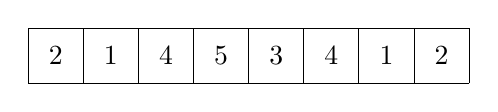
\begin{tikzpicture}[scale=0.7]
\draw (0,0) grid (8,1);

\node at (0.5,0.5) {$2$};
\node at (1.5,0.5) {$1$};
\node at (2.5,0.5) {$4$};
\node at (3.5,0.5) {$5$};
\node at (4.5,0.5) {$3$};
\node at (5.5,0.5) {$4$};
\node at (6.5,0.5) {$1$};
\node at (7.5,0.5) {$2$};
\end{tikzpicture}
\end{center}

Giả sử kích thước của cửa sổ trượt là 4.
Tại vị trí cửa sổ đầu tiên, giá trị nhỏ nhất là 1:
\begin{center}
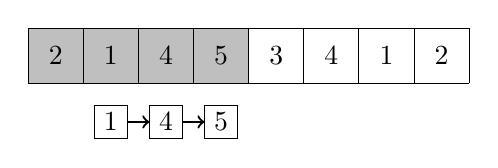
\begin{tikzpicture}[scale=0.7]
\fill[color=lightgray] (0,0) rectangle (4,1);
\draw (0,0) grid (8,1);

\node at (0.5,0.5) {$2$};
\node at (1.5,0.5) {$1$};
\node at (2.5,0.5) {$4$};
\node at (3.5,0.5) {$5$};
\node at (4.5,0.5) {$3$};
\node at (5.5,0.5) {$4$};
\node at (6.5,0.5) {$1$};
\node at (7.5,0.5) {$2$};

\draw (1.2,0.2-1.2) rectangle (1.8,0.8-1.2);
\draw (2.2,0.2-1.2) rectangle (2.8,0.8-1.2);
\draw (3.2,0.2-1.2) rectangle (3.8,0.8-1.2);

\node at (1.5,0.5-1.2) {$1$};
\node at (2.5,0.5-1.2) {$4$};
\node at (3.5,0.5-1.2) {$5$};

\draw[->,thick] (1.8,0.5-1.2) -- (2.2,0.5-1.2);
\draw[->,thick] (2.8,0.5-1.2) -- (3.2,0.5-1.2);
\end{tikzpicture}
\end{center}

Sau đó cửa sổ di chuyển một bước sang phải.
Phần tử mới 3 nhỏ hơn các phần tử
4 và 5 trong hàng đợi, vì vậy các phần tử 4 và 5
bị loại bỏ khỏi hàng đợi
và phần tử 3 được thêm vào hàng đợi.
Giá trị nhỏ nhất vẫn là 1.
\begin{center}
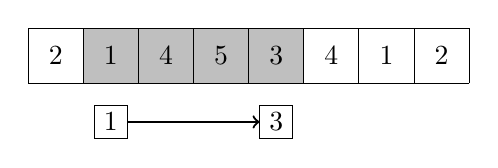
\begin{tikzpicture}[scale=0.7]
\fill[color=lightgray] (1,0) rectangle (5,1);
\draw (0,0) grid (8,1);

\node at (0.5,0.5) {$2$};
\node at (1.5,0.5) {$1$};
\node at (2.5,0.5) {$4$};
\node at (3.5,0.5) {$5$};
\node at (4.5,0.5) {$3$};
\node at (5.5,0.5) {$4$};
\node at (6.5,0.5) {$1$};
\node at (7.5,0.5) {$2$};

\draw (1.2,0.2-1.2) rectangle (1.8,0.8-1.2);
\draw (4.2,0.2-1.2) rectangle (4.8,0.8-1.2);

\node at (1.5,0.5-1.2) {$1$};
\node at (4.5,0.5-1.2) {$3$};

\draw[->,thick] (1.8,0.5-1.2) -- (4.2,0.5-1.2);
\end{tikzpicture}
\end{center}

Sau đó, cửa sổ lại di chuyển,
và phần tử nhỏ nhất 1
không còn thuộc cửa sổ nữa.
Do đó, nó bị loại bỏ khỏi hàng đợi và giá trị nhỏ nhất
bây giờ là 3. Phần tử mới 4 cũng
được thêm vào hàng đợi.
\begin{center}
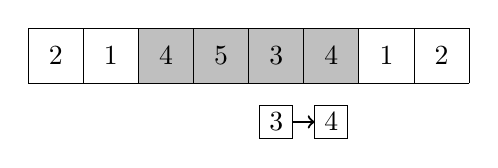
\begin{tikzpicture}[scale=0.7]
\fill[color=lightgray] (2,0) rectangle (6,1);
\draw (0,0) grid (8,1);

\node at (0.5,0.5) {$2$};
\node at (1.5,0.5) {$1$};
\node at (2.5,0.5) {$4$};
\node at (3.5,0.5) {$5$};
\node at (4.5,0.5) {$3$};
\node at (5.5,0.5) {$4$};
\node at (6.5,0.5) {$1$};
\node at (7.5,0.5) {$2$};

\draw (4.2,0.2-1.2) rectangle (4.8,0.8-1.2);
\draw (5.2,0.2-1.2) rectangle (5.8,0.8-1.2);

\node at (4.5,0.5-1.2) {$3$};
\node at (5.5,0.5-1.2) {$4$};

\draw[->,thick] (4.8,0.5-1.2) -- (5.2,0.5-1.2);
\end{tikzpicture}
\end{center}

Phần tử mới tiếp theo 1 nhỏ hơn tất cả các phần tử
trong hàng đợi.
Do đó, tất cả các phần tử bị loại bỏ khỏi hàng đợi
và nó sẽ chỉ chứa phần tử 1:
\begin{center}
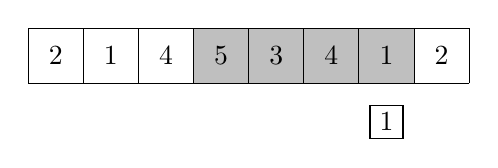
\begin{tikzpicture}[scale=0.7]
\fill[color=lightgray] (3,0) rectangle (7,1);
\draw (0,0) grid (8,1);

\node at (0.5,0.5) {$2$};
\node at (1.5,0.5) {$1$};
\node at (2.5,0.5) {$4$};
\node at (3.5,0.5) {$5$};
\node at (4.5,0.5) {$3$};
\node at (5.5,0.5) {$4$};
\node at (6.5,0.5) {$1$};
\node at (7.5,0.5) {$2$};

\draw (6.2,0.2-1.2) rectangle (6.8,0.8-1.2);

\node at (6.5,0.5-1.2) {$1$};
\end{tikzpicture}
\end{center}

Cuối cùng cửa sổ đạt đến vị trí cuối cùng của nó.
Phần tử 2 được thêm vào hàng đợi,
nhưng giá trị nhỏ nhất bên trong cửa sổ
vẫn là 1.
\begin{center}
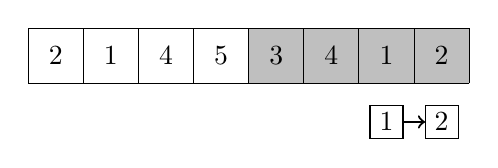
\begin{tikzpicture}[scale=0.7]
\fill[color=lightgray] (4,0) rectangle (8,1);
\draw (0,0) grid (8,1);

\node at (0.5,0.5) {$2$};
\node at (1.5,0.5) {$1$};
\node at (2.5,0.5) {$4$};
\node at (3.5,0.5) {$5$};
\node at (4.5,0.5) {$3$};
\node at (5.5,0.5) {$4$};
\node at (6.5,0.5) {$1$};
\node at (7.5,0.5) {$2$};

\draw (6.2,0.2-1.2) rectangle (6.8,0.8-1.2);
\draw (7.2,0.2-1.2) rectangle (7.8,0.8-1.2);

\node at (6.5,0.5-1.2) {$1$};
\node at (7.5,0.5-1.2) {$2$};

\draw[->,thick] (6.8,0.5-1.2) -- (7.2,0.5-1.2);
\end{tikzpicture}
\end{center}

Vì mỗi phần tử của mảng
được thêm vào hàng đợi đúng một lần và
bị loại bỏ khỏi hàng đợi nhiều nhất một lần,
thuật toán hoạt động trong thời gian $O(n)$.